% !TEX encoding = UTF-8
% !TEX TS-program = pdflatex
% !TEX root = ../tesi.tex

%**************************************************************
\chapter{Analisi dei requisiti}
\label{cap:analisi-requisiti}
%**************************************************************

Questo capitolo descrive i casi d'uso e i requisiti della piattaforma moviORDER, individuati e classificati per definire nel dettaglio obiettivi e funzionalità del sistema. I casi d'uso e i requisiti sono stati dedotti da un'analisi preliminare eseguita dal tutor aziendale, la quale è stata perfezionata dallo stagista per perseguire massima efficienza ed efficacia del sistema. Le convenzioni adottate per la stesura di casi d'uso e requisiti sono presenti in Appendice §\ref{}.

\section{Casi d'uso}

Per lo studio dei casi di utilizzo della piattaforma sono stati creati dei diagrammi dei casi d'uso che meglio descrivono funzioni e/o servizi offerti dal sistema, così come sono percepiti e utilizzati dagli attori che interagiscono con il sistema stesso. Per la definizione dei diagrammi UML dei casi d'uso è stato utilizzato lo standard UML 2.0.

\subsection{Attori del sistema}

Lo scopo di moviORDER è permettere alle aziende che forniscono dei prodotti di vendere gli stessi ai propri clienti tramite un'applicazione multipiattaforma. Quindi moviORDER viene distribuita da VISIONEIMPRESA alle aziende che forniscono prodotti, la quale viene distribuita dalle aziende stesse ai propri clienti. Gli utilizzatori finali di moviORDER sono quindi i clienti delle singole aziende che sono clienti di VISIONEIMPRESA.
L'accesso all'applicazione è consentito solamente agli utenti provvisti di credenziali di accesso, le quali vengono distribuite, insieme all'applicazione, dal fornitore. Non è prevista quindi una funzionalità di registrazione. Nel contesto di moviORDER vi sono quindi due tipologie di attori:
\begin{enumerate}
	\item \textbf{Utente non autenticato}: è un utente che non ha effettuato l'accesso al sistema al quale viene offerta la sola funzionalità di autenticazione. Una volta che un utente non autenticato viene riconosciuto accedendo al sistema, diventa un utente autenticato;
	\item \textbf{Utente autenticato}: è un utente che ha effettuato l'accesso al sistema e che può usufruire di tutte le sue funzionalità. Le funzionalità offerte all'utente autenticato sono:
	\begin{itemize}
		\item possibilità di effettuare il logout;
		\item possibilità di aggiungere articoli al proprio carrello;
		\item possibilità di modificare gli articoli nel proprio carrello;
		\item possibilità di rimuovere articoli dal proprio carrello;
		\item possibilità di inviare un ordine alla propria azienda.
	\end{itemize}
\end{enumerate}

\subsection{UC1 - Azioni utente non autenticato}

\begin{figure}[!h] 
    \centering 
    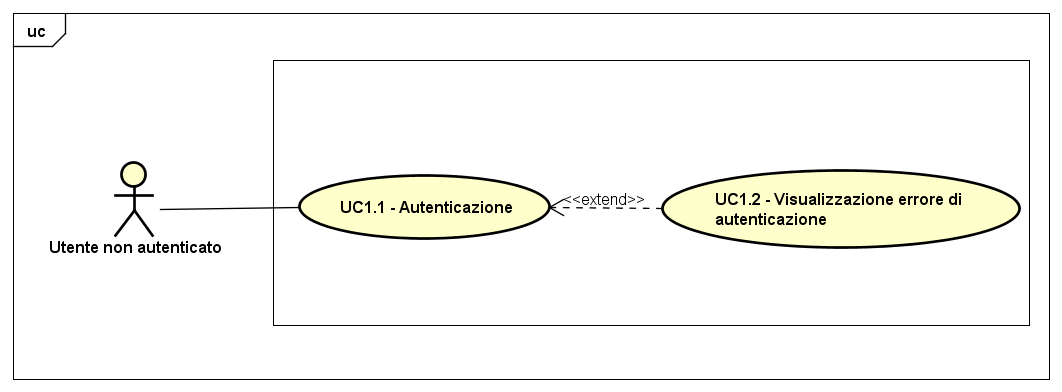
\includegraphics[width=0.9\columnwidth]{usecase/generaleNonAutenticato} 
    \caption{Use Case - UC1: Azioni utente non autenticato}
\end{figure}

\begin{itemize}
	\item \textbf{Attore}: Utente non autenticato;
	\item \textbf{Descrizione}: L'attore può eseguire l'operazione di autenticazione alla piattaforma moviORDER;
	\item \textbf{Pre-condizioni}: L'attore ha avviato l'applicazione e non è ancora stato riconosciuto dal sistema;
	\item \textbf{Post-condizioni}: L'attore ha eseguito l'operazione che desiderava compiere da utente non autenticato;
	\item \textbf{Scenario principale}: UC1.1 - Autenticazione;
	\item \textbf{Scenario alternativo}: L'attore ha fornito credenziali di accesso non corrispondenti a nessun utente registrato dall'azienda, oppure non riesce ad accedere al sistema perché è stato bloccato dall'azienda stessa: UC1.2 - Visualizzazione errore di autenticazione. 
\end{itemize}

\subsection{UC1.1 - Autenticazione}

\begin{figure}[!h] 
    \centering 
    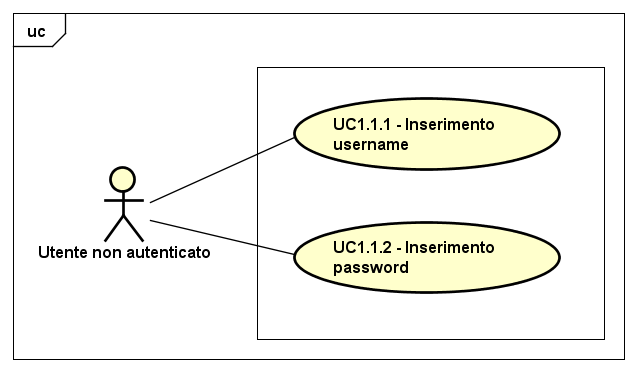
\includegraphics[width=0.9\columnwidth]{usecase/autenticazione} 
    \caption{Use Case - UC1.1: Autenticazione}
\end{figure}

\begin{itemize}
	\item \textbf{Attore}: Utente non autenticato;
	\item \textbf{Descrizione}: L'attore può eseguire l'operazione di autenticazione;
	\item \textbf{Pre-condizioni}: L'attore ha avviato l'applicazione, non è ancora riconosciuto dal sistema e ha espresso la volontà di effettuare l’autenticazione a moviORDER;
	\item \textbf{Post-condizioni}: L'attore ha eseguito l'operazione di accesso al sistema ed è quindi ora riconosciuto come utente autenticato;
	\item \textbf{Scenario principale}: 
		\begin{enumerate}
			\item UC1.1.1 - Inserimento username;
			\item UC1.1.2 - Inserimento password.
		\end{enumerate} 
\end{itemize}

\subsection{UC1.1.1 - Inserimento username}

\begin{itemize}
	\item \textbf{Attore}: Utente non autenticato;
	\item \textbf{Descrizione}: L'attore deve inserire una username per l'operazione di autenticazione;
	\item \textbf{Pre-condizioni}: L'attore ha avviato l'applicazione, non è ancora riconosciuto dal sistema e il sistema richiede l'inserimento di una username per l'operazione di autenticazione;
	\item \textbf{Post-condizioni}: L'attore ha inserito la username per l'operazione di autenticazione;
	\item \textbf{Scenario principale}: L'attore inserisce la username tramite una text box.
\end{itemize}

\subsection{UC1.1.2 - Inserimento password}

\begin{itemize}
	\item \textbf{Attore}: Utente non autenticato;
	\item \textbf{Descrizione}: L'attore deve inserire una password per l'operazione di autenticazione;
	\item \textbf{Pre-condizioni}: L'attore ha avviato l'applicazione, non è ancora riconosciuto dal sistema e il sistema richiede l'inserimento di una password per l'operazione di autenticazione;
	\item \textbf{Post-condizioni}: L'attore ha inserito la password per l'operazione di autenticazione;
	\item \textbf{Scenario principale}: L'attore inserisce la password tramite una text box.
\end{itemize}

\subsection{UC1.2 - Visualizzazione errore di autenticazione}

\begin{itemize}
	\item \textbf{Attore}: Utente non autenticato;
	\item \textbf{Descrizione}: L'attore inserisce credenziali di accesso non corrispondenti a nessun utente registrato dall'azienda, oppure l'utente è stato bloccato dall'azienda stessa;
	\item \textbf{Pre-condizioni}: L'attore ha avviato l'applicazione, non è ancora riconosciuto dal sistema e inserisce credenziali di accesso non corrispondenti a nessun utente registrato dall'azienda, oppure è stato bloccato;
	\item \textbf{Post-condizioni}: L'attore ha visualizzato un messaggio d'errore relativo all'impossibilità di eseguire l'autenticazione per inserimento di credenziali errate o perché è stato bloccato;
	\item \textbf{Scenario principale}: L'attore visualizza un messaggio d'errore relativo all'impossibilità di eseguire l'autenticazione per inserimento di credenziali errate o perché è stato bloccato.
\end{itemize}

\subsection{UC2 - Azioni utente autenticato}

\begin{figure}[!h] 
    \centering 
    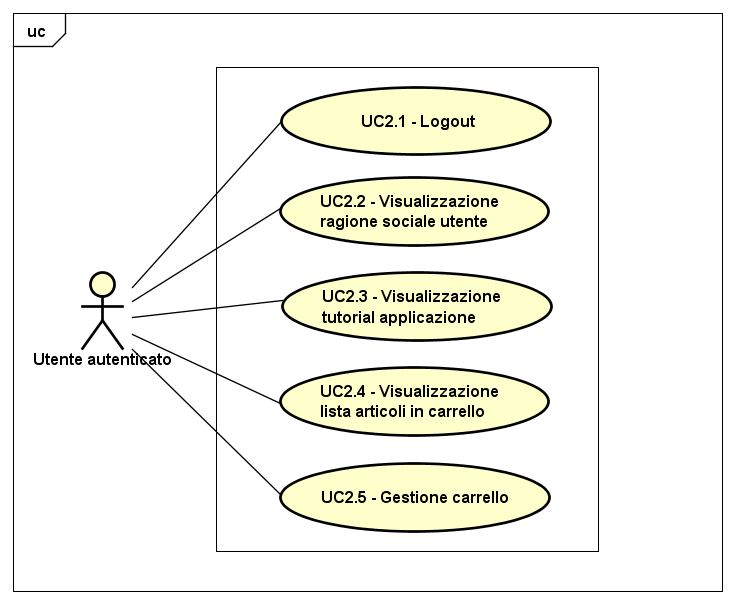
\includegraphics[width=0.9\columnwidth]{usecase/generaleAutenticato} 
    \caption{UC2 - Azioni utente autenticato}
\end{figure}

\begin{itemize}
	\item \textbf{Attore}: Utente autenticato;
	\item \textbf{Descrizione}: L'attore può:
	\begin{enumerate}
		\item eseguire l'operazione di logout;
		\item visualizzare il tutorial dell'applicazione;
		\item visualizzare la lista degli articoli in carrello;
		\item gestire il proprio carrello. 
	\end{enumerate}
	\item \textbf{Pre-condizioni}: L'attore ha avviato l'applicazione ed è riconosciuto dal sistema;
	\item \textbf{Post-condizioni}: L'attore ha eseguito le azioni che desiderava compiere da utente autenticato;
	\item \textbf{Scenario principale}: 
		\begin{enumerate}
			\item UC2.1 - Logout;
			\item UC2.2 - Visualizzazione tutorial applicazione;
			\item UC2.3 - Visualizzazione lista articoli in carrello;
			\item UC2.4 - Gestione carrello.
		\end{enumerate}
\end{itemize}

\subsection{UC2.1 - Logout}

\begin{itemize}
	\item \textbf{Attore}: Utente autenticato;
	\item \textbf{Descrizione}: L'attore può eseguire l'operazione di logout;
	\item \textbf{Pre-condizioni}: L'attore ha avviato l'applicazione, è riconosciuto dal sistema e ha espresso la volontà di effettuare il logout da moviORDER;
	\item \textbf{Post-condizioni}: L'attore ha eseguito l'operazione di logout da moviORDER ed è quindi uscito dal sistema tornando ad essere un utente non autenticato;
	\item \textbf{Scenario principale}: L'attore esegue l'operazione di logout da moviORDER premendo sul relativo bottone.
\end{itemize}

\subsection{UC2.2 - Visualizzazione tutorial applicazione}

\begin{itemize}
	\item \textbf{Attore}: Utente autenticato;
	\item \textbf{Descrizione}: L'attore può visualizzare il tutorial dell'applicazione;
	\item \textbf{Pre-condizioni}: L'attore ha avviato l'applicazione, è riconosciuto dal sistema e ha richiesto la visualizzazione del tutorial dell'applicazione;
	\item \textbf{Post-condizioni}: L'attore ha visualizzato il tutorial dell'applicazione;
	\item \textbf{Scenario principale}: L'attore visualizza il tutorial dell'applicazione premendo sul relativo bottone.
\end{itemize}

\subsection{UC2.3 - Gestione carrello}

\begin{figure}[!h] 
    \centering 
    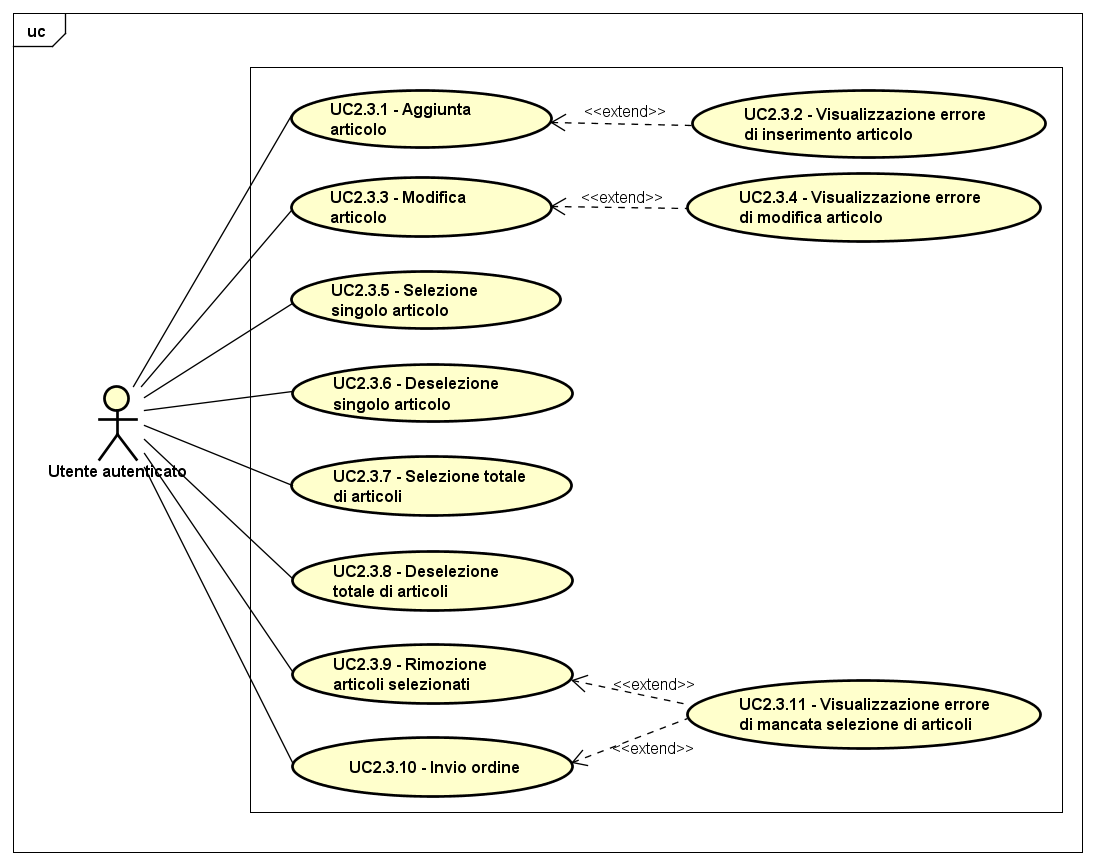
\includegraphics[width=0.9\columnwidth]{usecase/gestioneCarrello} 
    \caption{Use Case - UC1: Azioni utente non autenticato}
\end{figure}

\begin{itemize}
	\item \textbf{Attore}: Utente autenticato;
	\item \textbf{Descrizione}: L'attore può:
		\begin{enumerate}
			\item aggiungere un articolo al carrello;
			\item modificare un articolo in carrello;
			\item selezionare un singolo articolo in carrello;
			\item deselezionare un singolo articolo in carrello;
			\item selezionare tutti gli articoli in carrello;
			\item deselezionare tutti gli articoli in carrello;
			\item rimuovere articoli dal carrello;
			\item inviare un ordine.
		\end{enumerate}
	\item \textbf{Pre-condizioni}: L'attore ha avviato l'applicazione ed è riconosciuto dal sistema;
	\item \textbf{Post-condizioni}: L'attore ha eseguito le operazioni che desiderava compiere sul proprio carrello;
	\item \textbf{Scenario principale}:
		\begin{enumerate}
			\item UC2.3.1 - Aggiunta articolo;
			\item UC2.3.3 - Modifica articolo;
			\item UC2.3.5 - Selezione singolo articolo;
			\item UC2.3.6 - Deselezione singolo articolo;
			\item UC2.3.7 - Selezione totale di articoli;
			\item UC2.3.8 - Deselezione totale di articoli;
			\item UC2.3.9 - Rimozione articoli selezionati;
			\item UC2.3.10 - Invio ordine.
		\end{enumerate}
	\item \textbf{Scenari alternativi}:
		\begin{itemize}
			\item Durante l'operazione di aggiunta articolo, l'attore ha inserito un codice articolo non corrispondente a nessun articolo venduto dall'azienda, oppure ha inserito una quantità non permessa per l'articolo, oppure la scansione del codice a barre per la ricerca del codice articolo è fallita: UC2.3.2 - Visualizzazione errore di inserimento articolo;
			\item Durante l'operazione di modifica articolo, l'attore ha inserito una quantità non permessa per l'articolo: UC2.3.4 - Visualizzazione errore di modifica articolo;
			\item L'attore ha premuto il bottone di rimozione articoli selezionati senza aver selezionato alcun articolo dal carrello: UC2.3.11 - Visualizzazione errore di mancata selezione di articoli;
			\item L'attore ha premuto il bottone di invio ordine senza aver selezionato alcun articolo dal carrello: UC2.3.12 - Visualizzazione errore di mancata selezione di articoli.
		\end{itemize}
\end{itemize}

\subsection{UC2.3.1 - Aggiunta articolo}

\begin{figure}[!h] 
    \centering 
    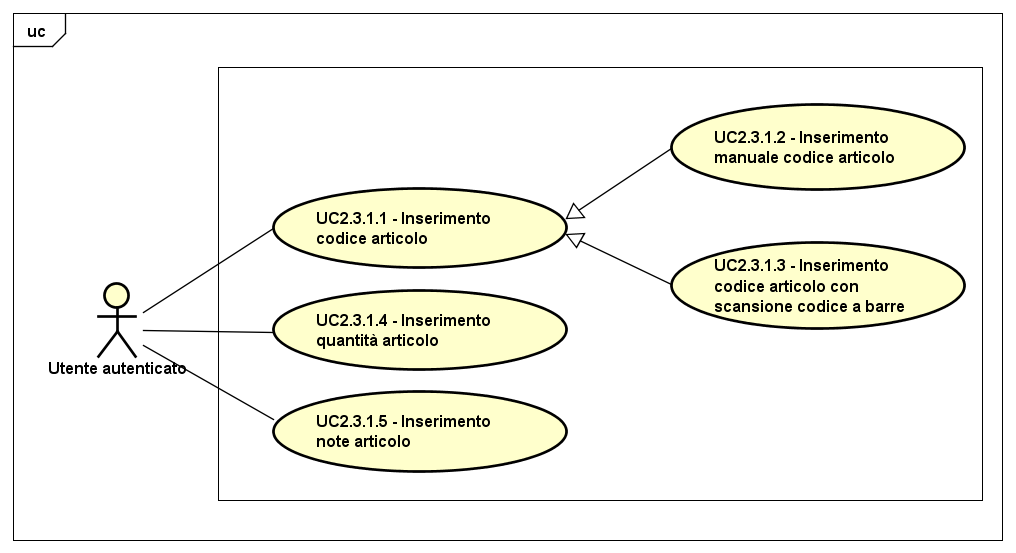
\includegraphics[width=0.9\columnwidth]{usecase/dettaglioAggiunta} 
    \caption{Use Case - UC1: Azioni utente non autenticato}
\end{figure}

\begin{itemize}
	\item \textbf{Attore}: Utente autenticato;
	\item \textbf{Descrizione}: L'attore può aggiungere un articolo al carrello;
	\item \textbf{Pre-condizioni}: L'attore ha avviato l'applicazione, è riconosciuto dal sistema e ha richiesto di aggiungere un articolo al carrello;
	\item \textbf{Post-condizioni}: L'attore ha aggiunto l'articolo al carrello;
	\item \textbf{Scenario principale}:
		\begin{enumerate}
			\item UC2.3.1.1 - Inserimento codice articolo;
			\item UC2.3.1.4 - Inserimento quantità articolo;
			\item UC2.3.1.5 - Inserimento note articolo.
		\end{enumerate}
\end{itemize}

\subsection{UC2.3.1.1 - Inserimento codice articolo}

\begin{itemize}
	\item \textbf{Attore}: Utente autenticato;
	\item \textbf{Descrizione}: L'attore deve inserire un codice articolo per l'operazione di aggiunta articolo;
	\item \textbf{Pre-condizioni}: L'attore ha avviato l'applicazione, è riconosciuto dal sistema, ha richiesto di aggiungere un articolo in carrello e il sistema richiede l'inserimento di un codice articolo per l'operazione di aggiunta articolo;
	\item \textbf{Post-condizioni}: L'attore ha inserito il codice articolo;
	\item \textbf{Scenario principale}: L'attore inserisce il codice articolo manualmente (UC2.3.1.2) o tramite la scansione di un codice a barre (UC2.3.1.3).
\end{itemize}

\subsection{UC2.3.1.2 - Inserimento manuale codice articolo}

\begin{itemize}
	\item \textbf{Attore}: Utente autenticato;
	\item \textbf{Descrizione}: L'attore deve inserire un codice articolo per l'operazione di aggiunta articolo;
	\item \textbf{Pre-condizioni}: L'attore ha avviato l'applicazione, è riconosciuto dal sistema, ha richiesto di aggiungere un articolo in carrello e quando il sistema richiede l'inserimento di un codice articolo per l'operazione di aggiunta articolo, l'attore esprime la volontà di voler inserire il codice articolo manualmente;
	\item \textbf{Post-condizioni}: L'attore ha inserito manualmente il codice articolo;
	\item \textbf{Scenario principale}: L'attore inserisce il codice articolo manualmente tramite una text box.
\end{itemize}

\subsection{UC2.3.1.3 - Inserimento codice articolo con scansione codice a barre}

\begin{itemize}
	\item \textbf{Attore}: Utente autenticato;
	\item \textbf{Descrizione}: L'attore deve inserire un codice articolo per l'operazione di aggiunta articolo;
	\item \textbf{Pre-condizioni}: L'attore ha avviato l'applicazione, è riconosciuto dal sistema, ha richiesto di aggiungere un articolo in carrello e quando il sistema richiede l'inserimento di un codice articolo per l'operazione di aggiunta articolo, l'attore esprime la volontà di voler inserire il codice articolo mediante la scansione del codice a barre di un articolo;
	\item \textbf{Post-condizioni}: L'attore ha inserito il codice articolo mediante la scansione del codice a barre dell'articolo;
	\item \textbf{Scenario principale}: L'attore inserisce il codice articolo mediante la scansione del codice a barre dell'articolo.
\end{itemize}

\subsection{UC2.3.1.4 - Inserimento quantità articolo}

\begin{itemize}
	\item \textbf{Attore}: Utente autenticato;
	\item \textbf{Descrizione}: L'attore deve inserire una quantità per l'operazione di aggiunta articolo;
	\item \textbf{Pre-condizioni}: L'attore ha avviato l'applicazione, è riconosciuto dal sistema, ha richiesto di aggiungere un articolo in carrello e il sistema richiede l'inserimento di una quantità per l'operazione di aggiunta articolo;
	\item \textbf{Post-condizioni}: L'attore ha inserito la quantità dell'articolo;
	\item \textbf{Scenario principale}: L'attore inserisce la quantità dell'articolo tramite una text box.
\end{itemize}

\subsection{UC2.3.1.5 - Inserimento note articolo}

\begin{itemize}
	\item \textbf{Attore}: Utente autenticato;
	\item \textbf{Descrizione}: L'attore può inserire delle note durante l'operazione di aggiunta articolo;
	\item \textbf{Pre-condizioni}: L'attore ha avviato l'applicazione, è riconosciuto dal sistema, ha richiesto di aggiungere un articolo in carrello e il sistema permette l'inserimento di note durante l'operazione di aggiunta articolo;
	\item \textbf{Post-condizioni}: L'attore ha inserito delle note per l'articolo;
	\item \textbf{Scenario principale}: L'attore inserisce delle note per l'articolo tramite una text area.
\end{itemize}

\subsection{UC2.3.2 - Visualizzazione errore di inserimento articolo}

\begin{itemize}
	\item \textbf{Attore}: Utente autenticato;
	\item \textbf{Descrizione}: L'attore inserisce un codice articolo non corrispondente a nessun articolo venduto dall'azienda, oppure inserisce una quantità non permessa per l'articolo, oppure la scansione del codice a barre per la ricerca del codice articolo è fallita;
	\item \textbf{Pre-condizioni}: L'attore ha avviato l'applicazione, è riconosciuto dal sistema, ha richiesto di aggiungere un articolo in carrello e ha inserito un codice articolo che non corrisponde a nessun articolo venduto dall'azienda, oppure ha inserito una quantità non permessa per l'articolo, oppure la scansione del codice a barre per la ricerca del codice articolo è fallita;
	\item \textbf{Post-condizioni}: L'attore ha visualizzato un messaggio d'errore relativo all'impossibilità di aggiungere l'articolo in carrello;
	\item \textbf{Scenario principale}: L'attore visualizza un messaggio d'errore relativo all'impossibilità di aggiungere l'articolo in carrello.
\end{itemize}

\subsection{UC2.3.3 - Modifica articolo}

\begin{figure}[!h] 
    \centering 
    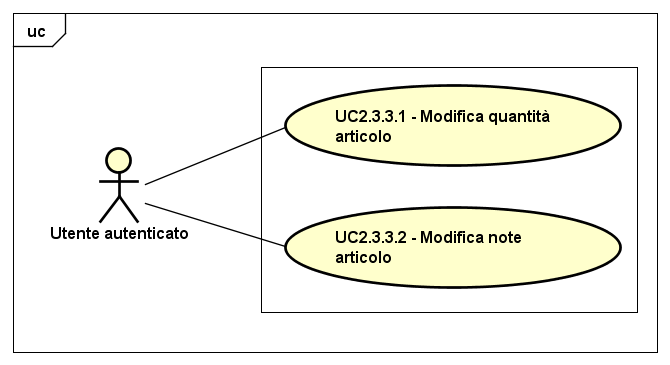
\includegraphics[width=0.9\columnwidth]{usecase/dettaglioModifica} 
    \caption{Use Case - UC1: Azioni utente non autenticato}
\end{figure}

\begin{itemize}
	\item \textbf{Attore}: Utente autenticato;
	\item \textbf{Descrizione}: L'attore può modificare un articolo in carrello;
	\item \textbf{Pre-condizioni}: L'attore ha avviato l'applicazione, è riconosciuto dal sistema e ha richiesto di modificare un articolo in carrello;
	\item \textbf{Post-condizioni}: L'attore ha modificato l'articolo in carrello;
	\item \textbf{Scenario principale}:
		\begin{enumerate}
			\item UC2.3.3.1 - Modifica quantità articolo;
			\item UC2.3.3.2 - Modifica note articolo.
		\end{enumerate}
\end{itemize}

\subsection{UC2.3.3.1 - Modifica quantità articolo}

\begin{itemize}
	\item \textbf{Attore}: Utente autenticato;
	\item \textbf{Descrizione}: L'attore può modificare la quantità dell'articolo selezionato;
	\item \textbf{Pre-condizioni}: L'attore ha avviato l'applicazione, è riconosciuto dal sistema, ha richiesto di modificare un articolo in carrello e il sistema permette la modifica della quantità dell'articolo selezionato;
	\item \textbf{Post-condizioni}: L'attore ha modificato la quantità dell'articolo selezionato;
	\item \textbf{Scenario principale}: L'attore modifica la quantità dell'articolo selezionato tramite una text box.
\end{itemize}

\subsection{UC2.3.3.2 - Modifica note articolo}

\begin{itemize}
	\item \textbf{Attore}: Utente autenticato;
	\item \textbf{Descrizione}: L'attore può modificare le note dell'articolo selezionato;
	\item \textbf{Pre-condizioni}: L'attore ha avviato l'applicazione, è riconosciuto dal sistema, ha richiesto di modificare un articolo in carrello e il sistema permette la modifica della note dell'articolo selezionato;
	\item \textbf{Post-condizioni}: L'attore ha modificato le note dell'articolo selezionato;
	\item \textbf{Scenario principale}: L'attore modifica le note dell'articolo selezionato tramite una text box.
\end{itemize}

\subsection{UC2.3.4 - Visualizzazione errore di modifica articolo}

\begin{itemize}
	\item \textbf{Attore}: Utente autenticato;
	\item \textbf{Descrizione}: L'attore inserisce una quantità non permessa per l'articolo selezionato;
	\item \textbf{Pre-condizioni}: L'attore ha avviato l'applicazione, è riconosciuto dal sistema, ha richiesto di modificare un articolo in carrello e ha inserito una quantità non permessa per l'articolo selezionato;
	\item \textbf{Post-condizioni}: L'attore ha visualizzato un messaggio d'errore relativo all'impossibilità di modificare l'articolo selezionato;
	\item \textbf{Scenario principale}: L'attore visualizza un messaggio d'errore relativo all'impossibilità di modificare l'articolo selezionato.
\end{itemize}

\subsection{UC2.3.5 - Selezione singolo articolo}

\begin{itemize}
	\item \textbf{Attore}: Utente autenticato;
	\item \textbf{Descrizione}: L'attore può selezionare un articolo non ancora selezionato in carrello;
	\item \textbf{Pre-condizioni}: L'attore ha avviato l'applicazione, è riconosciuto dal sistema e ha richiesto di selezionare un articolo non ancora selezionato in carrello;
	\item \textbf{Post-condizioni}: L'attore ha selezionato l'articolo in carrello;
	\item \textbf{Scenario principale}: L'attore seleziona l'articolo in carrello tramite una check-box.
\end{itemize}

\subsection{UC2.3.6 - Deselezione singolo articolo}

\begin{itemize}
	\item \textbf{Attore}: Utente autenticato;
	\item \textbf{Descrizione}: L'attore può deselezionare un articolo selezionato in carrello;
	\item \textbf{Pre-condizioni}: L'attore ha avviato l'applicazione, è riconosciuto dal sistema e ha richiesto di deselezionare un articolo selezionato in carrello;
	\item \textbf{Post-condizioni}: L'attore ha deselezionato l'articolo in carrello;
	\item \textbf{Scenario principale}: L'attore deseleziona l'articolo in carrello tramite una check-box.
\end{itemize}

\subsection{UC2.3.7 - Selezione totale di articoli}

\begin{itemize}
	\item \textbf{Attore}: Utente autenticato;
	\item \textbf{Descrizione}: L'attore può selezionare tutti gli articoli in carrello non ancora selezionati;
	\item \textbf{Pre-condizioni}: L'attore ha avviato l'applicazione, è riconosciuto dal sistema e ha richiesto di selezionare tutti gli articoli in carrello non ancora selezionati;
	\item \textbf{Post-condizioni}: L'attore ha selezionato tutti gli articoli in carrello non ancora selezionati;
	\item \textbf{Scenario principale}: L'attore seleziona tutti gli articoli in carrello non ancora selezionati premendo su un bottone.
\end{itemize}

\subsection{UC2.3.8 - Deselezione totale di articoli}

\begin{itemize}
	\item \textbf{Attore}: Utente autenticato;
	\item \textbf{Descrizione}: L'attore può deselezionare tutti gli articoli in carrello;
	\item \textbf{Pre-condizioni}: L'attore ha avviato l'applicazione, è riconosciuto dal sistema e ha richiesto di deselezionare tutti gli articoli in carrello;
	\item \textbf{Post-condizioni}: L'attore ha deselezionato tutti gli articoli in carrello;
	\item \textbf{Scenario principale}: L'attore deseleziona tutti gli articoli in carrello premendo su un bottone.
\end{itemize}

\subsection{UC2.3.9 - Rimozione articoli selezionati}

\begin{itemize}
	\item \textbf{Attore}: Utente autenticato;
	\item \textbf{Descrizione}: L'attore può rimuovere gli articoli selezionati dal carrello;
	\item \textbf{Pre-condizioni}: L'attore ha avviato l'applicazione, è riconosciuto dal sistema e ha richiesto di rimuovere gli articoli selezionati dal carrello;
	\item \textbf{Post-condizioni}: L'attore ha rimosso gli articoli selezionati dal carrello;
	\item \textbf{Scenario principale}: L'attore rimuove gli articoli selezionati dal carrello premendo su un bottone.
\end{itemize}

\subsection{UC2.3.10 - Invio ordine}

\begin{figure}[!h] 
    \centering 
    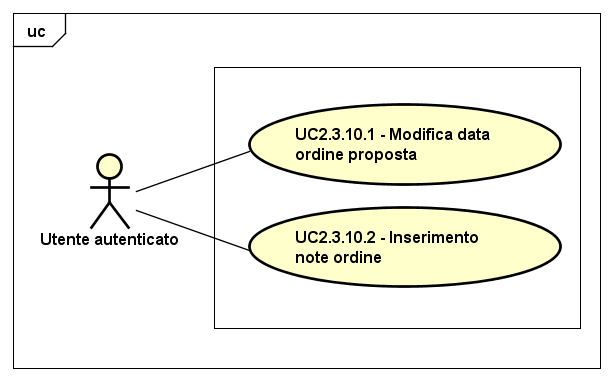
\includegraphics[width=0.9\columnwidth]{usecase/dettaglioInvioOrdine} 
    \caption{Use Case - UC1: Azioni utente non autenticato}
\end{figure}

\begin{itemize}
	\item \textbf{Attore}: Utente autenticato;
	\item \textbf{Descrizione}: L'attore può inviare un ordine composto dagli articoli selezionati in carrello;
	\item \textbf{Pre-condizioni}: L'attore ha avviato l'applicazione, è riconosciuto dal sistema e ha richiesto di inviare un ordine composto dagli articoli selezionati in carrello;
	\item \textbf{Post-condizioni}: L'attore ha inviato un ordine composto dagli articoli selezionati in carrello;
	\item \textbf{Scenario principale}:
		\begin{enumerate}
			\item UC2.3.10.1 - Modifica data ordine proposta;
			\item UC2.3.10.2 - Inserimento note ordine.
		\end{enumerate}
\end{itemize}

\subsection{UC2.3.10.1 - Modifica data ordine proposta}

\begin{itemize}
	\item \textbf{Attore}: Utente autenticato;
	\item \textbf{Descrizione}: L'attore può modificare la data d'ordine proposta;
	\item \textbf{Pre-condizioni}: L'attore ha avviato l'applicazione, è riconosciuto dal sistema, ha richiesto di inviare un ordine e il sistema permette la modifica della data d'ordine proposta;
	\item \textbf{Post-condizioni}: L'attore ha modificato la data d'ordine proposta;
	\item \textbf{Scenario principale}: L'attore modifica la data d'ordine proposta tramite una text box.
\end{itemize}

\subsection{UC2.3.10.2 - Inserimento note ordine}

\begin{itemize}
	\item \textbf{Attore}: Utente autenticato;
	\item \textbf{Descrizione}: L'attore può delle note per l'ordine;
	\item \textbf{Pre-condizioni}: L'attore ha avviato l'applicazione, è riconosciuto dal sistema, ha richiesto di inviare un ordine e il sistema permette l'inserimento di note per l'ordine;
	\item \textbf{Post-condizioni}: L'attore ha inserito le note per l'ordine;
	\item \textbf{Scenario principale}: L'attore le note per l'ordine tramite una text area.
\end{itemize}

\subsection{UC2.3.11 - Visualizzazione errore di mancata selezione di articoli}

\begin{itemize}
	\item \textbf{Attore}: Utente autenticato;
	\item \textbf{Descrizione}: L'attore preme sul bottone di rimozione articoli o invio ordine senza aver selezionato degli articoli in carrello;
	\item \textbf{Pre-condizioni}: L'attore ha avviato l'applicazione, è riconosciuto dal sistema, ha richiesto di rimuovere degli articoli dal carrello o di inviare un ordine, senza aver effettivamente selezionato degli articoli in carrello;
	\item \textbf{Post-condizioni}: L'attore ha visualizzato un messaggio d'errore relativo all'impossibilità di rimuovere gli articoli selezionati o inviare un ordine composto dagli articoli selezionati;
	\item \textbf{Scenario principale}: L'attore visualizza un messaggio d'errore relativo all'impossibilità di rimuovere gli articoli selezionati o inviare un ordine composto dagli articoli selezionati.
\end{itemize}

\section{Tracciamento dei requisiti}

Da un'attenta analisi dei requisiti e degli use case effettuata sul progetto è stata stilata la tabella che traccia i requisiti in rapporto agli use case.\\
Sono stati individuati diversi tipi di requisiti e si è quindi fatto utilizzo di un codice identificativo per distinguerli.\\
Il codice dei requisiti è così strutturato R(F/Q/V)(N/D/O) dove:
\begin{enumerate}
	\item[R =] requisito
    \item[F =] funzionale
    \item[Q =] qualitativo
    \item[V =] di vincolo
    \item[N =] obbligatorio (necessario)
    \item[D =] desiderabile
    \item[Z =] opzionale
\end{enumerate}
Nelle tabelle \ref{tab:requisiti-funzionali}, \ref{tab:requisiti-qualitativi} e \ref{tab:requisiti-vincolo} sono riassunti i requisiti e il loro tracciamento con gli use case delineati in fase di analisi.

\newpage

\begin{table}%
\caption{Tabella del tracciamento dei requisti funzionali}
\label{tab:requisiti-funzionali}
\begin{tabularx}{\textwidth}{lXl}
\hline\hline
\textbf{Requisito} & \textbf{Descrizione} & \textbf{Use Case}\\
\hline
RFN-1     & L'interfaccia permette di configurare il tipo di sonde del test & UC1 \\
\hline
\end{tabularx}
\end{table}%

\begin{table}%
\caption{Tabella del tracciamento dei requisiti qualitativi}
\label{tab:requisiti-qualitativi}
\begin{tabularx}{\textwidth}{lXl}
\hline\hline
\textbf{Requisito} & \textbf{Descrizione} & \textbf{Use Case}\\
\hline
RQD-1    & Le prestazioni del simulatore hardware deve garantire la giusta esecuzione dei test e non la generazione di falsi negativi & - \\
\hline
\end{tabularx}
\end{table}%

\begin{table}%
\caption{Tabella del tracciamento dei requisiti di vincolo}
\label{tab:requisiti-vincolo}
\begin{tabularx}{\textwidth}{lXl}
\hline\hline
\textbf{Requisito} & \textbf{Descrizione} & \textbf{Use Case}\\
\hline
RVO-1    & La libreria per l'esecuzione dei test automatici deve essere riutilizzabile & - \\
\hline
\end{tabularx}
\end{table}%